% !TEX encoding = UTF-8
% !TEX TS-program = pdflatex
% !TEX root = ../tesi.tex

%**************************************************************
\chapter{Analisi dei requisiti}
\label{cap:analisi-requisiti}
%**************************************************************

\intro{Il presente capitolo descrive in maniera dettagliata requisiti e casi
    d'uso individuati durante la fase di analisi del progetto di
    \textit{stage}.}\\

\section{Casi d'uso}
\subsection*{Attori principali}
Nella fase di analisi del progetto di \textit{stage} è emersa la presenza di un
solo attore, ovvero l'\textbf{utente autenticato},
attore che rappresenta un utente che ha effettuato l'autenticazione
all'interno della \textit{web app}. Questo attore ha la possibilità di
vedere
tutte le informazioni sui gruppi che sarebbero altrimenti inaccessibili.

\subsection*{Elenco dei casi d'uso}
Per lo studio dei casi di utilizzo del prodotto sono stati creati dei diagrammi
dei casi d'uso.
I diagrammi dei casi d'uso (in inglese \emph{Use Case Diagram}) sono diagrammi
di tipo \gls{uml} dedicati alla descrizione delle funzioni o servizi offerti da
un sistema, così come sono percepiti e utilizzati dagli attori che
interagiscono col sistema stesso.\\
I casi d'uso riportati in seguito descrivono solo le funzionalità che dovranno
essere implementate, senza quindi descrivere quelle già presenti nella
\textit{web app}.
\begin{figure}[H]
    \centering
    \includegraphics[width=1\columnwidth]{usecase/diagramma generale dei casi
        d'uso.png}
    \caption{Diagramma generale dei casi d'uso}
\end{figure}

\begin{usecase}{Visualizzazione lista dei gruppi}
    \label{uc:scenario-visualizzazione-lista-gruppi}
    \usecaseactors{Utente autenticato}
    \usecasepre{L'utente ha aperto la \textit{web app} ed è autenticato}
    \usecasedesc{L'utente vuole visualizzare la lista dei gruppi}
    \usecasepost{L'utente ha visualizzato la lista dei gruppi}
    \usecasescenarioprincipale{
        L'utente si trova nella schermata di visualizzazione della lista dei
        gruppi.
    }

\end{usecase}
\newpage

\begin{figure}[H]
    \centering
    \includegraphics[width=1.2\columnwidth]{usecase/sottocasi UC1.png}
    \caption{UC1: Vis. lista dei gruppi}
\end{figure}

\begin{subusecase}{Visualizzazione singolo gruppo in lista}
    \label{sub:visualizzazione-singolo-gruppo}
    \usecaseactors{Utente autenticato}
    \usecasepre{L'utente ha aperto la \textit{web app}, è autenticato e sta
        visualizzando la lista dei gruppi}
    \usecasedesc{L'utente vuole visualizzare un singolo gruppo nella lista dei
        gruppi}
    \usecasepost{L'utente ha visualizzato un singolo gruppo nella lista dei
        gruppi}
    \usecasescenarioprincipale{
        L'utente si trova nella schermata di visualizzazione dei gruppi e
        visualizza un singolo gruppo dalla lista dei gruppi.
    }
\end{subusecase}

\begin{figure}[H]
    \centering
    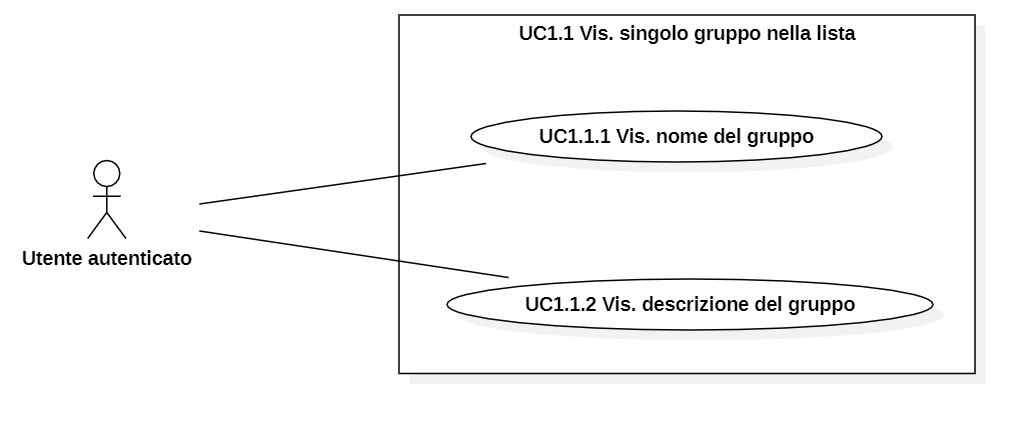
\includegraphics[width=1.2\columnwidth]{usecase/sottocasi UC1.1.png}
    \caption{UC1.1: Vis. singolo gruppo in lista}
\end{figure}

\newpage

\begin{subsubusecase}{Visualizzazione nome del gruppo}
    \label{subsub:visualizzazione-nome-gruppo}
    \usecaseactors{Utente autenticato}
    \usecasepre{L'utente ha aperto la \textit{web app}, è autenticato e sta
        visualizzando un gruppo dalla lista dei gruppi}
    \usecasedesc{L'utente vuole visualizzare il nome di un gruppo dalla lista
        dei gruppi}
    \usecasepost{L'utente ha visualizzato il nome di un gruppo dalla lista dei
        gruppi}
    \usecasescenarioprincipale{
        L'utente si trova nella schermata di visualizzazione dei gruppi e
        visualizza dalla lista dei gruppi il nome di uno specifico gruppo.
    }
\end{subsubusecase}

\begin{subsubusecase}{Visualizzazione descrizione del gruppo}
    \label{subsub:visualizzazione-descrizione-gruppo}
    \usecaseactors{Utente autenticato}
    \usecasepre{L'utente ha aperto la \textit{web app}, è autenticato e sta
        visualizzando un gruppo dalla lista dei gruppi}
    \usecasedesc{L'utente vuole visualizzare la descrizione di gruppo della
        lista dei gruppi}
    \usecasepost{L'utente ha visualizzato la descrizione di un gruppo dalla
        lista dei gruppi}
    \usecasescenarioprincipale{
        L'utente si trova nella schermata di visualizzazione dei gruppi
        evisualizza dalla lista dei gruppi la descrizione di uno specifico
        gruppo.
    }
\end{subsubusecase}

\begin{usecase}{Visualizzazione lista dei gruppi creati dall'utente}
    \label{uc:scenario-visualizzazione-lista-gruppi-creati}
    \usecaseactors{Utente autenticato}
    \usecasepre{L'utente ha aperto la \textit{web app} ed è autenticato}
    \usecasedesc{L'utente vuole visualizzare la lista dei gruppi creati da lui}
    \usecasepost{L'utente ha visualizzato la lista dei gruppi creati da lui}
    \usecasescenarioprincipale{
        L'utente si trova nella schermata di visualizzazione dei gruppi, in
        particolare la schermata dei gruppi creati dall'utente.
    }
\end{usecase}

\begin{usecase}{Visualizzazione lista dei gruppi a cui partecipa un utente}
    \label{uc:scenario-visualizzazione-lista-gruppi-partecipa}
    \usecaseactors{Utente autenticato}
    \usecasepre{L'utente ha aperto la \textit{web app} ed è autenticato}
    \usecasedesc{L'utente vuole visualizzare la lista dei gruppi a cui
        partecipa}
    \usecasepost{L'utente ha visualizzato la lista dei gruppi a cui partecipa}
    \usecasescenarioprincipale{
        L'utente si trova nella schermata di visualizzazione dei gruppi, in
        particolare la schermata dei gruppi a cui partecipa l'utente. I gruppi
        creati
        dall'utente, nonostante vi partecipi, non sono visualizzati in questa
        schermata.
    }
\end{usecase}

\begin{usecase}{Visualizzazione lista dei gruppi creati da altri utenti}
    \label{uc:scenario-visualizzazione-lista-gruppi-altri}
    \usecaseactors{Utente autenticato}
    \usecasepre{L'utente ha aperto la \textit{web app} ed è autenticato}
    \usecasedesc{L'utente vuole visualizzare la lista dei gruppi creati da
        altri utenti}
    \usecasepost{L'utente ha visualizzato la lista dei gruppi creati da altri
        utenti}
    \usecasescenarioprincipale{
        L'utente si trova nella schermata di visualizzazione dei gruppi, in
        particolare la schermata dei gruppi creati da altri utenti a cui è
        possibile
        partecipare. Non sono quindi presenti in questa schermata i gruppi a
        cui partecipa già un utente.
    }
\end{usecase}

\begin{usecase}{Visualizzazione dettagli di un gruppo}
    \label{uc:scenario-visualizzazione-dettaglio-gruppo}
    \usecaseactors{Utente autenticato}
    \usecasepre{L'utente ha aperto la \textit{web app}, è autenticato e sta
        visualizzando la lista dei gruppi}
    \usecasedesc{L'utente vuole visualizzare i dettagli di un gruppo}
    \usecasepost{L'utente ha visualizzato i dettagli di un gruppo}
    \usecasescenarioprincipale{
        L'utente, che si trova nella schermata di visualizzazione dei gruppi,
        decide di visualizzare i dettagli di un gruppo.
    }
\end{usecase}
\begin{figure}[H]
    \centering
    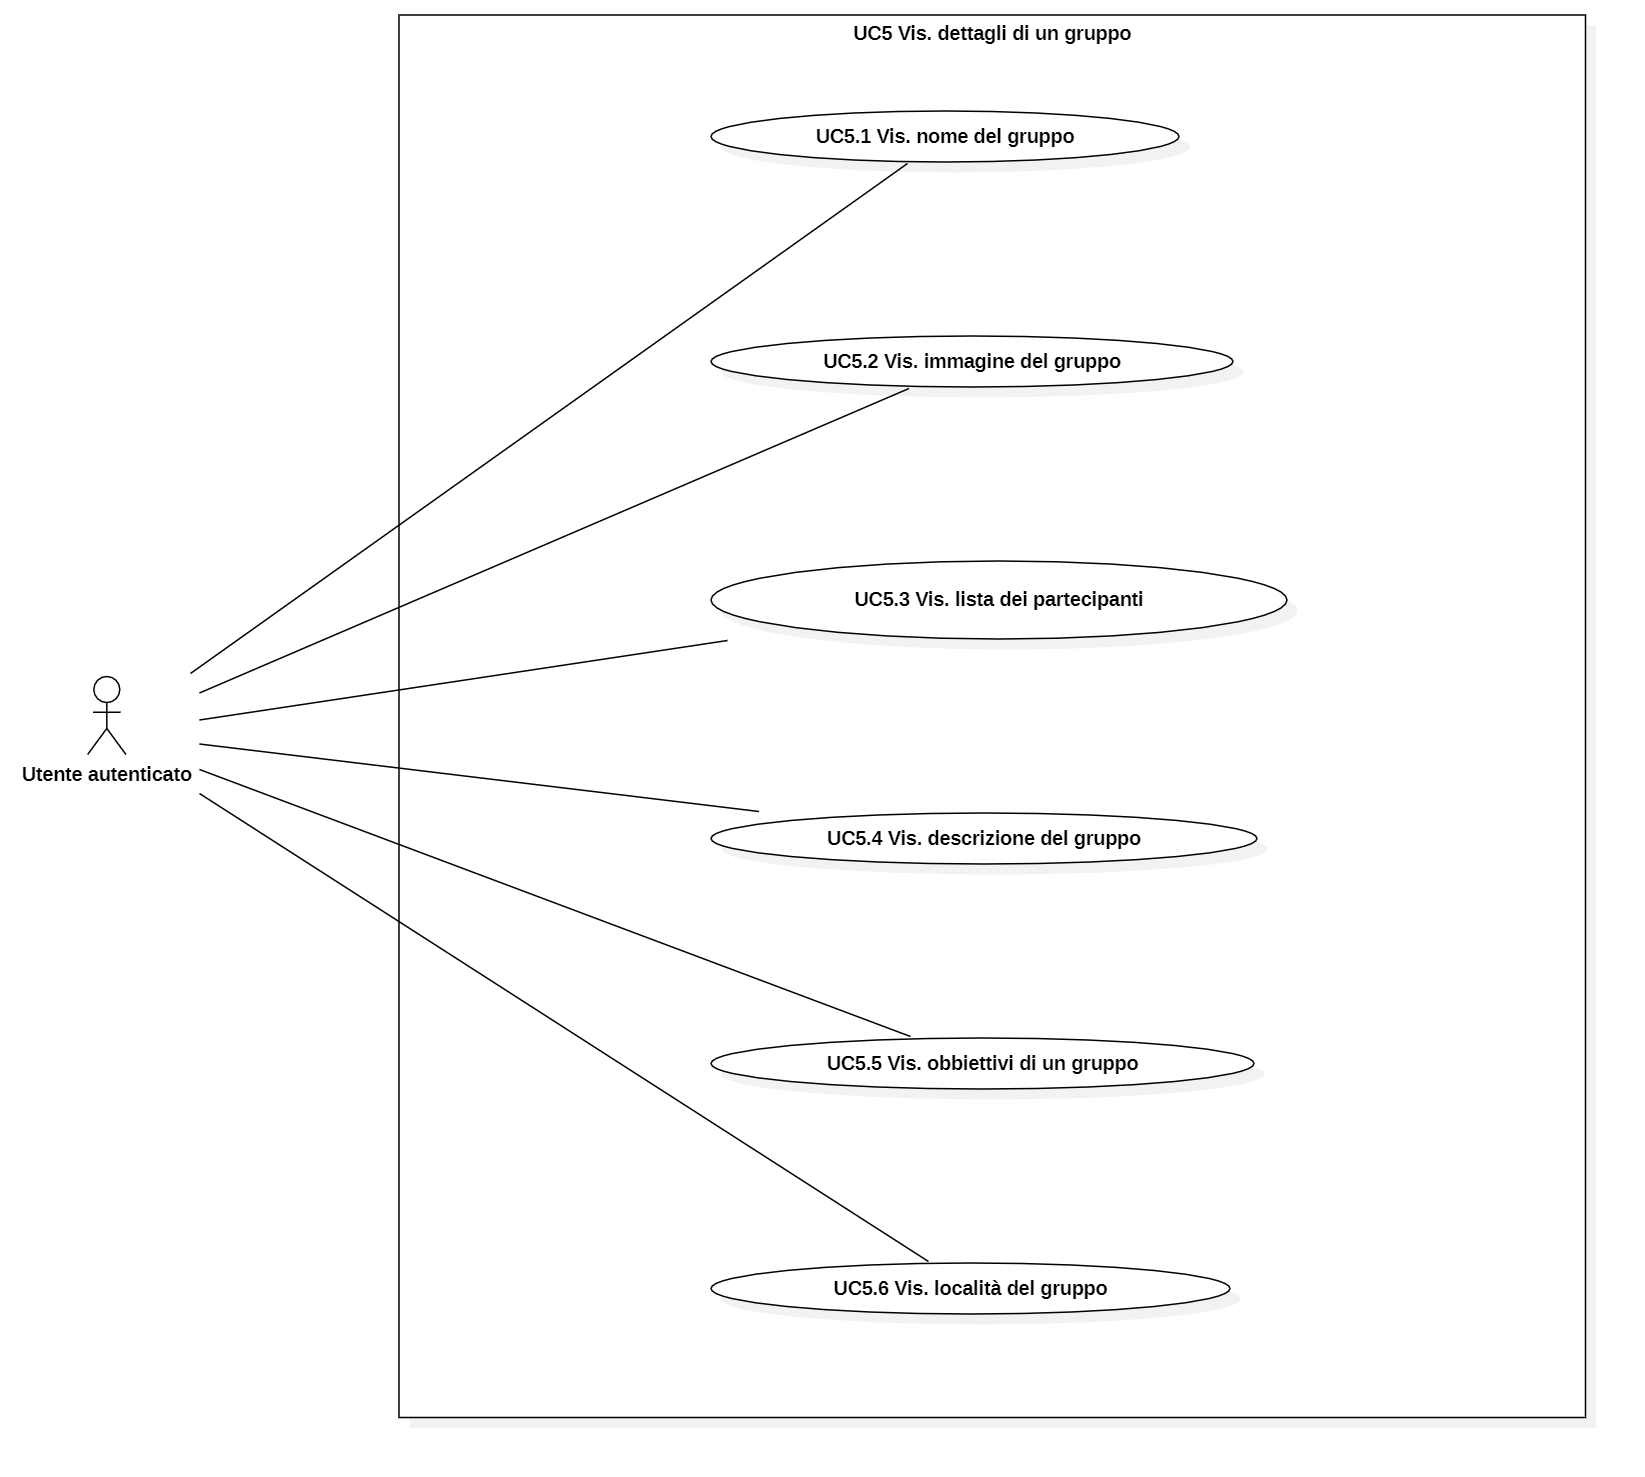
\includegraphics[width=0.85\columnwidth]{usecase/sottocasi UC5.png}
    \caption{UC5: Vis. dettagli di un gruppo}
\end{figure}
\newpage

\begin{subusecase}{Visualizzazione nome del gruppo}
    \label{sub:visualizzazione-nome-gruppo}
    \usecaseactors{Utente autenticato}
    \usecasepre{L'utente ha aperto la \textit{web app}, è autenticato e sta
        visualizzando i dettagli di un gruppo}
    \usecasedesc{L'utente vuole visualizzare il nome di un gruppo}
    \usecasepost{L'utente ha visualizzato il nome di un gruppo}
    \usecasescenarioprincipale{
        L'utente dalla schermata dei gruppi ha deciso di visualizzare i
        dettagli di un gruppo, e dalla schermata di visualizzazione dei
        dettagli di un gruppo visualizza il nome del gruppo.
    }
\end{subusecase}

\begin{subusecase}{Visualizzazione immagine del gruppo}
    \label{sub:visualizzazione-immagine-gruppo}
    \usecaseactors{Utente autenticato}
    \usecasepre{L'utente ha aperto la \textit{web app}, è autenticato e sta
        visualizzando i dettagli di un gruppo}
    \usecasedesc{L'utente vuole visualizzare l'immagine di un gruppo}
    \usecasepost{L'utente ha visualizzato l'immagine di un gruppo}
    \usecasescenarioprincipale{
        L'utente dalla schermata dei gruppi ha deciso di visualizzare i
        dettagli di un gruppo, e dalla schermata di visualizzazione dei
        dettagli di un gruppo visualizza l'immagine del
        gruppo.
    }
\end{subusecase}

\begin{subusecase}{Visualizzazione lista dei partecipanti di un gruppo}
    \label{sub:visualizzazione-utenti-gruppo}
    \usecaseactors{Utente autenticato}
    \usecasepre{L'utente ha aperto la \textit{web app}, è autenticato e sta
        visualizzando i dettagli di un gruppo}
    \usecasedesc{L'utente vuole visualizzare la lista dei partecipanti ad un
        gruppo}
    \usecasepost{L'utente ha visualizzato la lista dei partecipanti ad un
        gruppo}
    \usecasescenarioprincipale{
        L'utente dalla schermata dei gruppi ha deciso di visualizzare i
        dettagli di un gruppo, e dalla schermata di visualizzazione dei
        dettagli di un gruppo visualizza	la lista dei
        partecipanti ad un gruppo.
    }
\end{subusecase}

\begin{figure}[H]
    \centering
    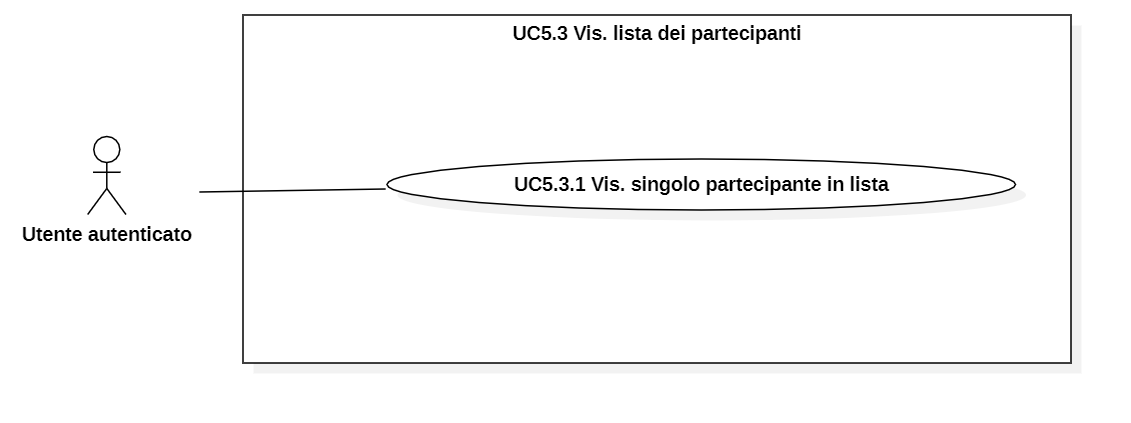
\includegraphics[width=1\columnwidth]{usecase/sottocasi UC5.3.png}
    \caption{UC5.3: Vis. lista dei partecipanti di un gruppo}
\end{figure}

\begin{subsubusecase}{Visualizzazione singolo partecipante in lista}
    \label{subsub:visualizzazione-partecipanti-gruppo}
    \usecaseactors{Utente autenticato}
    \usecasepre{L'utente ha aperto la \textit{web app}, è autenticato e sta
        visualizzando la lista dei partecipanti ad un gruppo}
    \usecasedesc{L'utente vuole visualizzare un partecipante dalla lista dei
        partecipanti ad un gruppo}
    \usecasepost{L'utente ha visualizzato un partecipante dalla lista dei
        partecipanti ad un gruppo}
    \usecasescenarioprincipale{
        L'utente dalla schermata dei gruppi ha deciso di visualizzare i
        dettagli di un gruppo, e dalla schermata di visualizzazione dei
        dettagli di un gruppo visualizza	un partecipante dalla
        lista dei
        partecipanti ad un gruppo.
    }
\end{subsubusecase}

\begin{figure}[H]
    \centering
    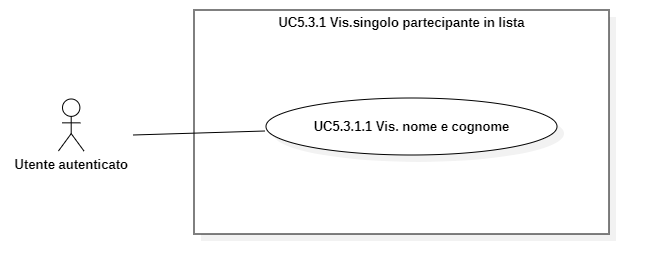
\includegraphics[width=1\columnwidth]{usecase/sottocasi UC5.3.1.png}
    \caption{UC5.3.1: Vis. singolo partecipante in lista}
\end{figure}

\begin{subsubsubusecase}{Visualizzazione singolo partecipante in lista}
    \label{subsubsub:visualizzazione-singolo-partecipante-gruppo}
    \usecaseactors{Utente autenticato}
    \usecasepre{L'utente ha aperto la \textit{web app}, è autenticato e sta
        visualizzando un partecipante dalla lista dei partecipanti}
    \usecasedesc{L'utente vuole visualizzare nome e cognome di un partecipante
        dalla lista dei partecipanti}
    \usecasepost{L'utente ha visualizzato nome e cognome di un partecipante
        dalla lista dei partecipanti}
    \usecasescenarioprincipale{
        L'utente dalla schermata dei gruppi ha deciso di visualizzare i
        dettagli di un gruppo, e dalla schermata di visualizzazione dei
        dettagli di un gruppo visualizza	il nome e il cognome di
        un
        partecipante dalla lista dei partecipanti ad un gruppo.
    }
\end{subsubsubusecase}

\begin{subusecase}{Visualizzazione descrizione del gruppo}
    \label{sub:visualizzazione-descrizione-gruppo}
    \usecaseactors{Utente autenticato}
    \usecasepre{L'utente ha aperto la \textit{web app}, è autenticato e sta
        visualizzando i dettagli di un gruppo}
    \usecasedesc{L'utente vuole visualizzare la descrizione di un gruppo}
    \usecasepost{L'utente ha visualizzato la descrizione di un gruppo}
    \usecasescenarioprincipale{
        L'utente dalla schermata dei gruppi ha deciso di visualizzare i
        dettagli di un gruppo, e dalla schermata di visualizzazione dei
        dettagli di un gruppo visualizza	la descrizione di un
        gruppo.
    }
\end{subusecase}

\begin{subusecase}{Visualizzazione obiettivi del gruppo}
    \label{sub:visualizzazione-obiettivi-gruppo}
    \usecaseactors{Utente autenticato}
    \usecasepre{L'utente ha aperto la \textit{web app}, è autenticato e sta
        visualizzando i dettagli di un gruppo}
    \usecasedesc{L'utente vuole visualizzare gli obiettivi di un gruppo}
    \usecasepost{L'utente ha visualizzato gli obiettivi di un gruppo}
    \usecasescenarioprincipale{
        L'utente dalla schermata dei gruppi ha deciso di visualizzare i
        dettagli di un gruppo, e dalla schermata di visualizzazione dei
        dettagli di un gruppo visualizza gli obiettivi di un
        gruppo.
    }
\end{subusecase}

\begin{subusecase}{Visualizzazione località del gruppo}
    \label{sub:visualizzazione-località-gruppo}
    \usecaseactors{Utente autenticato}
    \usecasepre{L'utente ha aperto la \textit{web app}, è autenticato e sta
        visualizzando i dettagli di un gruppo}
    \usecasedesc{L'utente vuole visualizzare la località di un gruppo}
    \usecasepost{L'utente ha visualizzato la località di un gruppo}
    \usecasescenarioprincipale{
        L'utente dalla schermata dei gruppi ha deciso di visualizzare i
        dettagli di un gruppo, e dalla schermata di visualizzazione dei
        dettagli di un gruppo visualizza la località in cui il
        gruppo è presente.
    }
\end{subusecase}

\begin{usecase}{Modifica di un gruppo}
    \label{uc:scenario-modifica-gruppo}
    \usecaseactors{Utente autenticato}
    \usecasepre{L'utente ha aperto la \textit{web app}, è autenticato e sta
        visualizzando la lista dei gruppi creati da lui}
    \usecasedesc{L'utente vuole modificare i dettagli di un gruppo}
    \usecasepost{L'utente ha modificato i dettagli di un gruppo}
    \usecasescenarioprincipale{
        L'utente si trova nella schermata di visualizzazione dei gruppi, in
        particolare dei gruppi creati dall'utente e desidera modificare i
        dettagli di un gruppo dalla schermata di modifica dei gruppi.
    }
\end{usecase}

\begin{figure}[H]
    \centering
    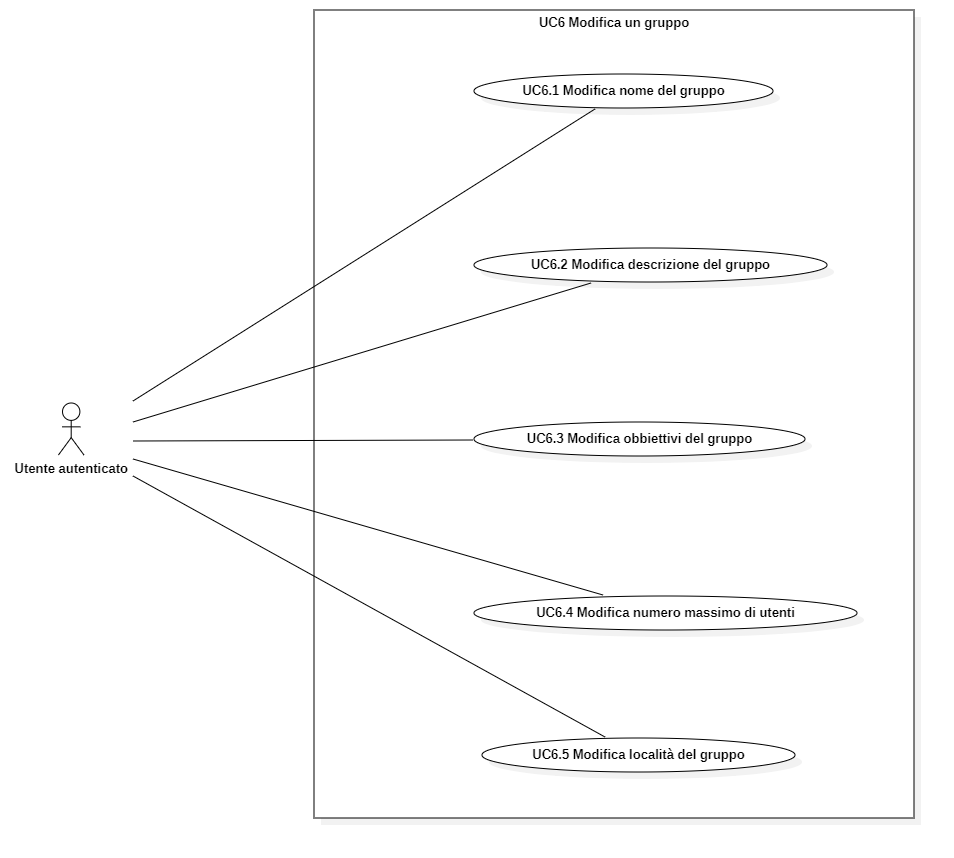
\includegraphics[width=0.8\columnwidth]{usecase/sottocasi UC6.png}
    \caption{UC6: Modifica di un gruppo}
\end{figure}

\begin{subusecase}{Modifica nome del gruppo}
    \label{sub:modifica-nome-gruppo}
    \usecaseactors{Utente autenticato}
    \usecasepre{L'utente ha aperto la \textit{web app}, è autenticato e sta
        modificando i dettagli di un gruppo}
    \usecasedesc{L'utente vuole modificare il nome di un gruppo}
    \usecasepost{L'utente ha modificato il nome di un gruppo}
    \usecasescenarioprincipale{
        L'utente si trova nella schermata di visualizzazione dei gruppi, in
        particolare dei gruppi creati dall'utente e desidera modificare il nome
        di un gruppo dalla schermata di modifica dei gruppi.
    }
\end{subusecase}

\begin{subusecase}{Modifica descrizione del gruppo}
    \label{sub:modifica-descrizione-gruppo}
    \usecaseactors{Utente autenticato}
    \usecasepre{L'utente ha aperto la \textit{web app}, è autenticato e sta
        modificando i dettagli di un gruppo}
    \usecasedesc{L'utente vuole modificare la descrizione di un gruppo}
    \usecasepost{L'utente ha modificato la descrizione di un gruppo}
    \usecasescenarioprincipale{
        L'utente si trova nella schermata di visualizzazione dei gruppi, in
        particolare dei gruppi creati dall'utente e desidera modificare la
        descrizione di un gruppo dalla schermata di modifica dei gruppi.
    }
\end{subusecase}

\begin{subusecase}{Modifica obiettivi del gruppo}
    \label{sub:modifica-obiettivi-gruppo}
    \usecaseactors{Utente autenticato}
    \usecasepre{L'utente ha aperto la \textit{web app}, è autenticato e sta
        modificando i dettagli di un gruppo}
    \usecasedesc{L'utente vuole modificare gli obiettivi di un gruppo}
    \usecasepost{L'utente ha modificato gli obiettivi di un gruppo}
    \usecasescenarioprincipale{
        L'utente si trova nella schermata di visualizzazione dei gruppi, in
        particolare dei gruppi creati dall'utente e desidera modificare gli
        obiettivi di un gruppo dalla schermata di modifica dei gruppi.
    }
\end{subusecase}

\begin{subusecase}{Modifica numero massimo di utenti}
    \label{sub:modifica-numero-utenti-gruppo}
    \usecaseactors{Utente autenticato}
    \usecasepre{L'utente ha aperto la \textit{web app}, è autenticato e sta
        modificando i dettagli di un gruppo}
    \usecasedesc{L'utente vuole modificare il numero massimo di utenti di un
        gruppo}
    \usecasepost{L'utente ha modificato il numero massimo di utenti di un
        gruppo}
    \usecasescenarioprincipale{
        L'utente si trova nella schermata di visualizzazione dei gruppi, in
        particolare dei gruppi creati dall'utente e desidera modificare il
        numero massimo di partecipanti ad un gruppo dalla schermata di
        modifica. Nel caso al gruppo vi partecipino più utenti di quanto
        modificato, non sarà più permesso ad altri utenti unirsi al gruppo.
    }
\end{subusecase}

\begin{subusecase}{Modifica località del gruppo}
    \label{sub:modifica-località-gruppo}
    \usecaseactors{Utente autenticato}
    \usecasepre{L'utente ha aperto la \textit{web app}, è autenticato e sta
        modificando i dettagli di un gruppo}
    \usecasedesc{L'utente vuole modificare la località di un gruppo}
    \usecasepost{L'utente ha modificato la località di un gruppo}
    \usecasescenarioprincipale{
        L'utente si trova nella schermata di visualizzazione dei gruppi, in
        particolare dei gruppi creati dall'utente e desidera modificare la
        località in cui è presente un gruppo dalla schermata di modifica dei
        gruppi.
    }
\end{subusecase}
% TODO: se resta tempo implementare questa funzionalità
% \begin{subusecase}{Rimozione utente}
%     \label{sub:rimozione-utente}
%     \usecaseactors{Utente autenticato}
%     \usecasepre{L'utente ha aperto la \textit{web app}, è autenticato e sta modificando i dettagli di un gruppo}
%     \usecasedesc{L'utente vuole rimuovere un utente dal gruppo}
%     \usecasepost{L'utente ha rimosso un utente dal gruppo}
%     \usecasescenarioprincipale{
%         \begin{enumerate}[nolistsep]
%             \item L'utente visualizza la lista dei gruppi;
%             \item l'utente clicca su un gruppo sul che vuole modificare;
%             \item l'utente rimuove un utente dal gruppo.
%         \end{enumerate}
%     }
% \end{subusecase}

\begin{usecase}{Crea un nuovo gruppo}
    \label{uc:scenario-creazione-nuovo-gruppo}
    \usecaseactors{Utente autenticato}
    \usecasepre{L'utente ha aperto la \textit{web app} ed è autenticato}
    \usecasedesc{L'utente vuole creare un nuovo gruppo}
    \usecasepost{L'utente ha creato un nuovo gruppo}
    \usecasescenarioprincipale{
        L'utente si trova nella schermata di visualizzazione dei gruppi, in
        particolare dei gruppi creati dall'utente e crea un nuovo
        gruppo dalla schermata di creazione di un gruppo.
    }
\end{usecase}

\begin{figure}[H]
    \centering
    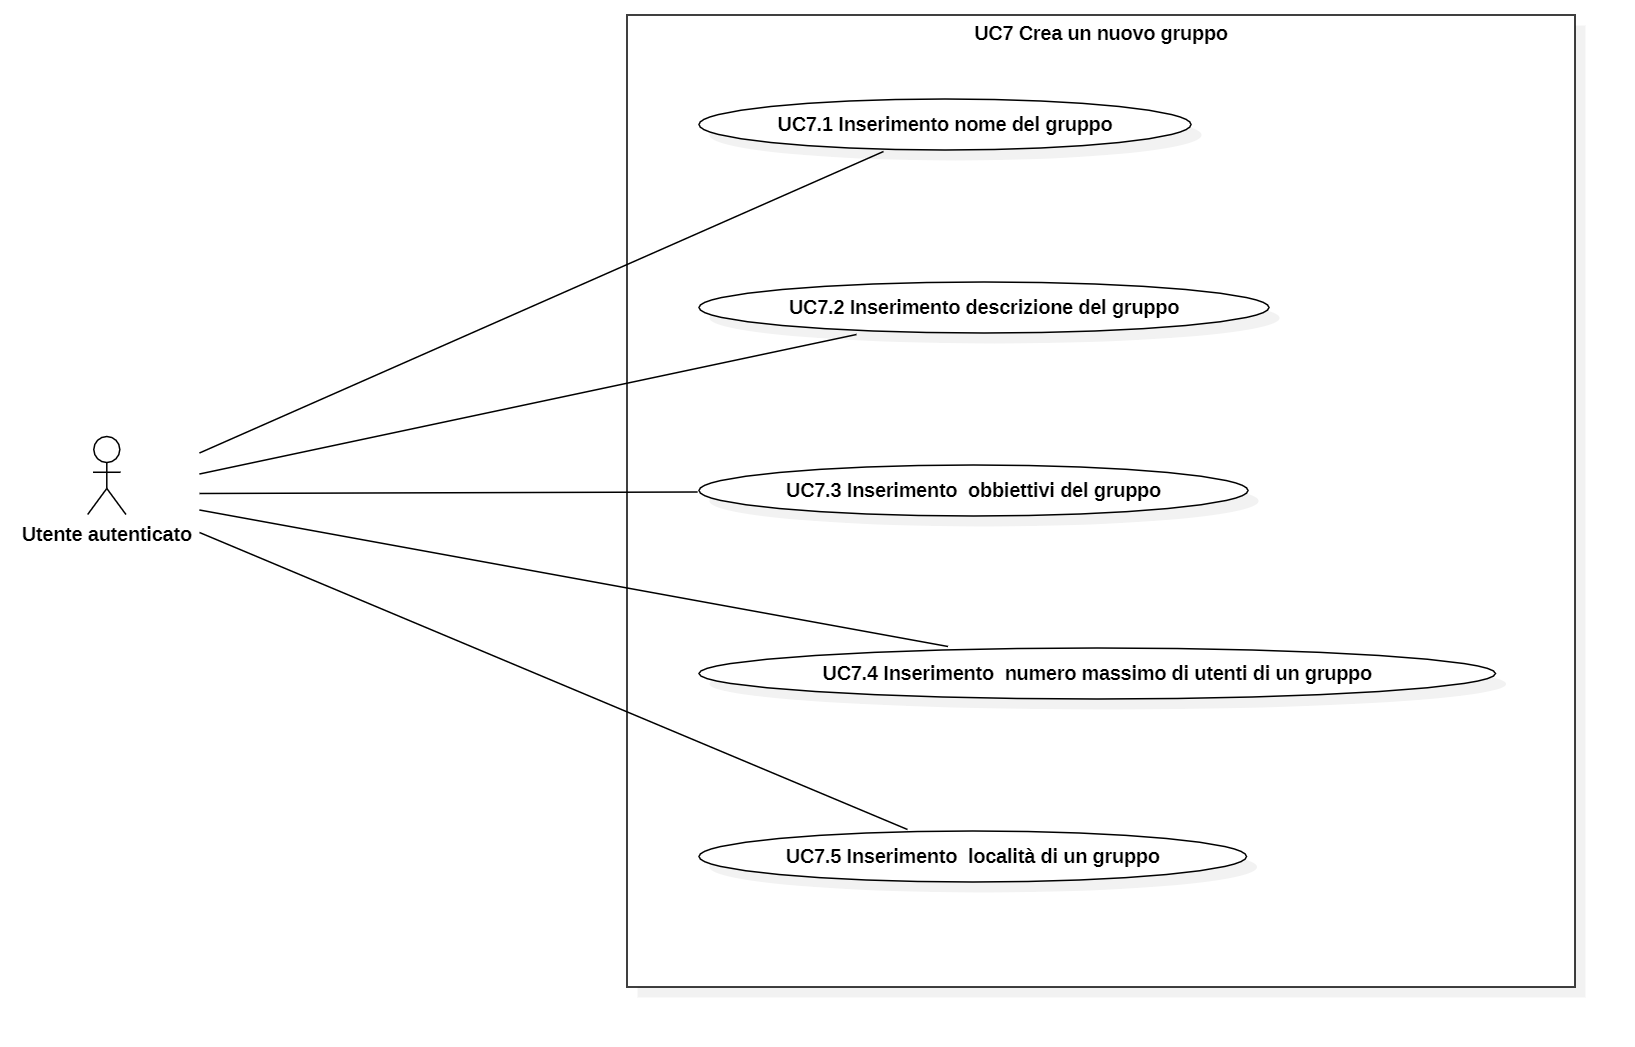
\includegraphics[width=1\columnwidth]{usecase/sottocasi UC7.png}
    \caption{UC7: Crea un nuovo gruppo}
\end{figure}

\begin{subusecase}{Inserimento nome del gruppo}
    \label{sub:inserimento-nome-gruppo}
    \usecaseactors{Utente autenticato}
    \usecasepre{L'utente ha aperto la \textit{web app}, è autenticato e sta
        creando un nuovo gruppo}
    \usecasedesc{L'utente vuole inserire il nome del gruppo}
    \usecasepost{L'utente ha inserito il nome del gruppo}
    \usecasescenarioprincipale{
        L'utente si trova nella schermata di visualizzazione dei gruppi, in
        particolare dei gruppi creati dall'utente e inserisce il nome
        del gruppo dalla schermata di creazione di un gruppo.
    }
\end{subusecase}

\begin{subusecase}{Inserimento descrizione del gruppo}
    \label{sub:inserimento-descrizione-gruppo}
    \usecaseactors{Utente autenticato}
    \usecasepre{L'utente ha aperto la \textit{web app}, è autenticato e sta
        creando un nuovo gruppo}
    \usecasedesc{L'utente vuole inserire la descrizione del gruppo}
    \usecasepost{L'utente ha inserito la descrizione del gruppo}
    \usecasescenarioprincipale{
        L'utente si trova nella schermata di visualizzazione dei gruppi, in
        particolare dei gruppi creati dall'utente e inserisce la
        descrizione del gruppo dalla schermata di creazione di un gruppo.
    }
\end{subusecase}

\begin{subusecase}{Inserimento obiettivi del gruppo}
    \label{sub:inserimento-obiettivi-gruppo}
    \usecaseactors{Utente autenticato}
    \usecasepre{L'utente ha aperto la \textit{web app}, è autenticato e sta
        creando un nuovo gruppo}
    \usecasedesc{L'utente vuole inserire gli obiettivi del gruppo}
    \usecasepost{L'utente ha inserito gli obiettivi del gruppo}
    \usecasescenarioprincipale{
        L'utente si trova nella schermata di visualizzazione dei gruppi, in
        particolare dei gruppi creati dall'utente e inserisce gli
        obiettivi del gruppo dalla schermata di creazione di un gruppo.
    }
\end{subusecase}

\begin{subusecase}{Inserimento numero massimo di utenti nel gruppo}
    \label{sub:inserimento-numero-utenti-gruppo}
    \usecaseactors{Utente autenticato}
    \usecasepre{L'utente ha aperto la \textit{web app}, è autenticato e sta
        creando un nuovo gruppo}
    \usecasedesc{L'utente vuole inserire il numero massimo di utenti del
        gruppo}
    \usecasepost{L'utente ha inserito il numero massimo di utenti del gruppo}
    \usecasescenarioprincipale{
        L'utente si trova nella schermata di visualizzazione dei gruppi, in
        particolare dei gruppi creati dall'utente e inserisce il numero
        massimo di partecipanti al gruppo dalla schermata di creazione di un
        gruppo.
    }
\end{subusecase}

\begin{subusecase}{Inserimento località del gruppo}
    \label{sub:inserimento-località-gruppo}
    \usecaseactors{Utente autenticato}
    \usecasepre{L'utente ha aperto la \textit{web app}, è autenticato e sta
        creando un nuovo gruppo}
    \usecasedesc{L'utente vuole inserire la località del gruppo}
    \usecasepost{L'utente ha inserito la località del gruppo}
    \usecasescenarioprincipale{
        L'utente si trova nella schermata di visualizzazione dei gruppi, in
        particolare dei gruppi creati dall'utente e inserisce la
        località in cui è presente il gruppo dalla schermata di creazione di un
        gruppo.
    }
\end{subusecase}

\begin{usecase}{Elimina un gruppo}
    \label{uc:scenario-elimina-gruppo}
    \usecaseactors{Utente autenticato}
    \usecasepre{L'utente ha aperto la \textit{web app}, è autenticato e si
        trova nella pagina di modifica di un gruppo}
    \usecasedesc{L'utente vuole eliminare un gruppo}
    \usecasepost{L'utente ha eliminato un gruppo}
    \usecasescenarioprincipale{
        L'utente si trova nella schermata di modifica dei gruppi di un gruppo
        creato
        dall'utente ed elimina il gruppo in questione.
    }
\end{usecase}

\begin{usecase}{Partecipa ad un gruppo}
    \label{uc:scenario-partecipa-gruppo}
    \usecaseactors{Utente autenticato}
    \usecasepre{L'utente ha aperto la \textit{web app}, è autenticato e si
        trova nella pagina dei dettagli di un gruppo a cui non partecipa}
    \usecasedesc{L'utente vuole partecipare ad un gruppo}
    \usecasepost{L'utente ha partecipato al gruppo}
    \usecasescenarioprincipale{
        L'utente si trova nella schermata dei dettagli di un  gruppo a cui
        non partecipa, e partecipa al gruppo in questione.
    }
\end{usecase}

% \begin{usecase}{Visualizzazione errore numero di utenti massimo raggiunto}
%     \label{uc:errore-numero-utenti}
%     \usecaseactors{Utente autenticato}
%     \usecasepre{L'utente ha aperto la \textit{web app} ed è autenticato}
%     \usecasedesc{L'utente vuole partecipare ad un gruppo}
%     \usecasepost{L'utente non si unisce al gruppo}
%     \usecasescenarioprincipale{
%         \begin{enumerate}[nolistsep]
%             \item l'utente sceglie di partecipare ad un gruppo;
%             \item viene visualizzato un messaggio di errore a causa della capienza massima raggiunta dal gruppo.
%         \end{enumerate}
%     }
% \end{usecase}

\begin{usecase}{Annulla partecipazione ad un gruppo}
    \label{uc:scenario-annulla-partecipazione}
    \usecaseactors{Utente autenticato}
    \usecasepre{L'utente ha aperto la \textit{web app}, è autenticato e si
        trova nella pagina dei dettagli di un gruppo a cui partecipa}
    \usecasedesc{L'utente vuole annullare la partecipazione al gruppo}
    \usecasepost{L'utente ha annullato la partecipazione al gruppo}
    \usecasescenarioprincipale{
        L'utente si trova nella schermata dei dettagli di un  gruppo a cui
        già partecipa, e annulla la partecipazione al gruppo in questione.
    }
\end{usecase}

\begin{usecase}{Visualizzazione lista delle will degli utenti appartenenti agli
        stessi gruppi}
    \label{uc:scenario-visualizzazione-will}
    \usecaseactors{Utente autenticato}
    \usecasepre{L'utente ha aperto la \textit{web app} ed è autenticato}
    \usecasedesc{L'utente vuole visualizzare la lista delle \gls{will} degli
        utenti appartenenti agli stessi gruppi}
    \usecasepost{L'utente ha visualizzato la lista delle \gls{will} degli
        utenti appartenenti agli stessi gruppi}
    \usecasescenarioprincipale{
        L'utente si trova nella schermata principale della \textit{web app}
        nella finestra di visualizzazione della lista delle \gls{will} degli
        utenti
        appartenenti agli stessi gruppi a cui partecipa l'utente.
    }
\end{usecase}

\begin{figure}[H]
    \centering
    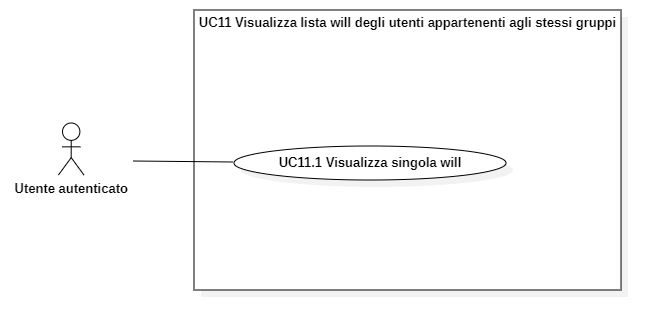
\includegraphics[width=1.2\columnwidth]{usecase/sottocasi UC11.png}
    \caption{UC11: Vis. lista \textit{will} degli utenti appartenenti agli
        stessi gruppi}
\end{figure}

\begin{subusecase}{Visualizzazione singola will in lista}
    \label{sub:visualizzazione-singola-will}
    \usecaseactors{Utente autenticato}
    \usecasepre{L'utente ha aperto la \textit{web app}, è autenticato e sta
        visualizzando la lista delle \gls{will}}
    \usecasedesc{L'utente vuole visualizzare una singola \gls{will} dalla lista
        delle \gls{will}}
    \usecasepost{L'utente ha visualizzato una singola \gls{will} dalla lista
        delle \gls{will}}
    \usecasescenarioprincipale{
        L'utente si trova nella schermata principale della \textit{web app},
        nella finestra di visualizzazione dalla
        lista
        delle \gls{will} degli utenti appartenenti agli stessi gruppi a cui
        partecipa l'utente e visualizza una \gls{will} da questa lista.
    }
\end{subusecase}

\begin{figure}[H]
    \centering
    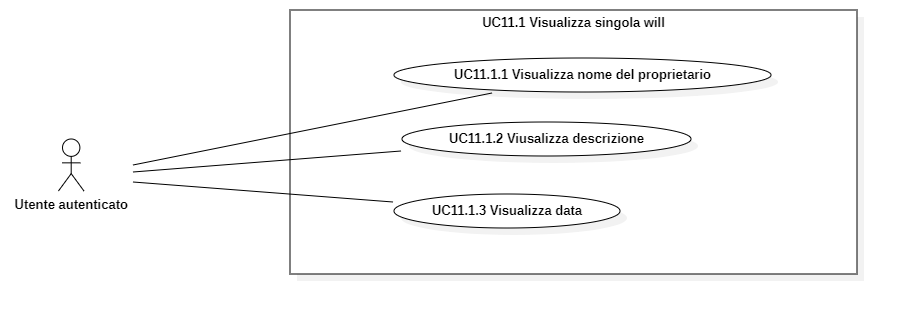
\includegraphics[width=1.2\columnwidth]{usecase/sottocasi UC11.1.png}
    \caption{UC11.1: Vis. singola \textit{will}}
\end{figure}

\begin{subsubusecase}{Visualizzazione nome del proprietario}
    \label{subsub:visualizzazione-will-nome-proprietario}
    \usecaseactors{Utente autenticato}
    \usecasepre{L'utente ha aperto la \textit{web app}, è autenticato e sta
        visualizzando un \gls{will} dalla lista delle \gls{will}}
    \usecasedesc{L'utente vuole visualizzare il nome del proprietario della
        \gls{will} dalla lista delle \gls{will}}
    \usecasepost{L'utente ha visualizzato il nome del proprietario della
        \gls{will} dalla lista delle \gls{will}}
    \usecasescenarioprincipale{
        L'utente si trova nella schermata principale della \textit{web app},
        nella finestra di visualizzazione dalla
        lista
        delle \gls{will} degli utenti appartenenti agli stessi gruppi a cui
        partecipa l'utente e visualizza il nome del proprietario di una
        \gls{will} dalla lista delle \gls{will}.
    }
\end{subsubusecase}

\begin{subsubusecase}{Visualizzazione descrizione}
    \label{subsub:visualizzazione-will-descrizione}
    \usecaseactors{Utente autenticato}
    \usecasepre{L'utente ha aperto la \textit{web app}, è autenticato e sta
        visualizzando un \gls{will} dalla lista delle \gls{will}}
    \usecasedesc{L'utente vuole visualizzare la descrizione della \gls{will}
        dalla lista delle \gls{will}}
    \usecasepost{L'utente ha visualizzato la descrizione della \gls{will} dalla
        lista delle \gls{will}}
    \usecasescenarioprincipale{
        L'utente si trova nella schermata principale della \textit{web app},
        nella finestra di visualizzazione dalla
        lista
        delle \gls{will} degli utenti appartenenti agli stessi gruppi a cui
        partecipa l'utente e visualizza la descrizione di una
        \gls{will} dalla lista delle \gls{will}.
    }
\end{subsubusecase}

\begin{subsubusecase}{Visualizzazione data}
    \label{subsub:visualizzazione-will-data}
    \usecaseactors{Utente autenticato}
    \usecasepre{L'utente ha aperto la \textit{web app}, è autenticato e sta
        visualizzando un \gls{will} dalla lista delle \gls{will}}
    \usecasedesc{L'utente vuole visualizzare la data in cui verrà effettuata
        l'uscita}
    \usecasepost{L'utente ha visualizzato la data in cui verrà effettuata
        l'uscita}
    \usecasescenarioprincipale{
        L'utente si trova nella schermata principale della \textit{web app},
        nella finestra di visualizzazione dalla
        lista
        delle \gls{will} degli utenti appartenenti agli stessi gruppi a cui
        partecipa l'utente e visualizza la data di uscita di una
        \gls{will} dalla lista delle \gls{will}.
    }
\end{subsubusecase}

\section{Tracciamento dei requisiti}
Da un'attenta analisi dei requisiti e degli \textit{use case} effettuata sul
progetto è
stata stilata la tabella che traccia i requisiti in rapporto agli \textit{use
    case}.\\
Sono stati individuati diversi tipi di requisiti e si è quindi fatto utilizzo
di un codice identificativo per distinguerli.\\
Il codice dei requisiti è così strutturato R(F/Q/V)(N/D/O) dove:
\begin{enumerate}[nolistsep]
    \item[R =] requisito
    \item[F =] funzionale
    \item[Q =] qualitativo
    \item[V =] di vincolo
    \item[N =] obbligatorio (necessario)
    \item[D =] desiderabile
    \item[Z =] opzionale
\end{enumerate}
Nelle tabelle \ref{tab:requisiti-funzionali}, \ref{tab:requisiti-qualitativi} e
\ref{tab:requisiti-vincolo} sono riassunti i requisiti e il loro tracciamento
con gli use case delineati in fase di analisi.

\begin{center}
  {\rowcolors{2}{color1}{color2}
    \renewcommand{\arraystretch}{1.3}
    \begin{longtable}{
      |>{\centering\arraybackslash}p{60pt}
      |>{\centering\arraybackslash}p{220pt}
      |>{\centering\arraybackslash}p{60pt}|}

      \rowcolor{antimaincolor!0}
      \caption{\label{tab:requisiti-funzionali}Tabella del tracciamento dei
      requisiti funzionali}                                                                                                                \\

      \hline
      \rowcolor{maincolor}
      \color{antimaincolor}{Requisito}
                                                                           &
      \color{antimaincolor}{Descrizione}
                                                                           &
      \color{antimaincolor}{Fonte}
      \\
      \hline
      \endhead

      \rowcolor{maincolor}
      \color{antimaincolor}{Requisito}
                                                                           &
      \color{antimaincolor}{Descrizione}
                                                                           &
      \color{antimaincolor}{Fonte}
      \\
      \hline
      \endfoot

      RFO-1                                                                & Il sistema deve permettere di visualizzare la lista dei
      gruppi                                                               & \nameref{uc:scenario-visualizzazione-lista-gruppi}            \\
      \hline
      RFO-1.1                                                              & Il sistema deve permettere di visualizzare un singolo
      gruppo nella lista dei gruppi                                        & \nameref{sub:visualizzazione-singolo-gruppo}                  \\
      \hline
      RFO-1.1.1                                                            & Il sistema deve permettere di visualizzare il nome di un
      gruppo dalla lista dei gruppi                                        & \nameref{subsub:visualizzazione-nome-gruppo}                  \\
      \hline
      RFO-1.1.2                                                            & Il sistema deve permettere di visualizzare la descrizione
      di un gruppo dalla lista dei gruppi                                  &
      \nameref{subsub:visualizzazione-descrizione-gruppo}                                                                                  \\
      \hline
      RFO-2                                                                & Il sistema deve permettere di visualizzare la lista dei
      gruppi creati dall'utente                                            &
      \nameref{uc:scenario-visualizzazione-lista-gruppi-creati}                                                                            \\
      \hline
      RFO-3                                                                & Il sistema deve permettere di visualizzare la lista dei
      gruppi	a cui partecipa l'utente                                       &
      \nameref{uc:scenario-visualizzazione-lista-gruppi-partecipa}                                                                         \\
      \hline
      RFO-4                                                                & Il sistema deve permettere di visualizzare la lista dei
      gruppi creati da altri utenti                                        &
      \nameref{uc:scenario-visualizzazione-lista-gruppi-altri}                                                                             \\
      \hline
      RFO-5                                                                & Il sistema deve permettere di visualizzare i dettagli di un
      gruppo                                                               & \nameref{uc:scenario-visualizzazione-dettaglio-gruppo}        \\
      \hline
      RFO-5.1                                                              & Il sistema deve permettere di visualizzare il nome di un
      gruppo                                                               & \nameref{sub:visualizzazione-nome-gruppo}                     \\
      \hline
      RFO-5.2                                                              & Il sistema deve permettere di visualizzare l'immagine di
      un gruppo                                                            & \nameref{sub:visualizzazione-immagine-gruppo}                 \\
      \hline

      RFO-5.3                                                              & Il sistema deve permettere di visualizzare la lista dei
      partecipanti ad un gruppo                                            & \nameref{sub:visualizzazione-utenti-gruppo}                   \\
      \hline

      RFO-5.3.1                                                            & Il sistema deve permettere di visualizzare un
      partecipante dalla lista dei partecipanti ad un gruppo               &
      \nameref{subsub:visualizzazione-partecipanti-gruppo}                                                                                 \\
      \hline

      RFO-5.3.1.1                                                          & Il sistema deve permettere di visualizzare nome e
      cognome di un partecipante dalla lista dei partecipanti ad un gruppo &
      \nameref{subsubsub:visualizzazione-singolo-partecipante-gruppo}                                                                      \\
      \hline

      RFO-5.4                                                              & Il sistema deve permettere di visualizzare la descrizione
      di un gruppo                                                         & \nameref{sub:visualizzazione-descrizione-gruppo}              \\
      \hline

      RFO-5.5                                                              & Il sistema deve permettere di visualizzare gli obbiettivi
      di un gruppo                                                         & \nameref{sub:visualizzazione-obbiettivi-gruppo}               \\
      \hline

      RFO-5.6                                                              & Il sistema deve permettere di visualizzare  località di
      un gruppo                                                            & \nameref{sub:visualizzazione-località-gruppo}                 \\
      \hline

      RFO-6                                                                & Il sistema deve permettere di modificare i dettagli di un
      gruppo                                                               & \nameref{uc:scenario-modifica-gruppo}                         \\
      \hline

      RFO-6.1                                                              & Il sistema deve permettere di modificare il nome di un
      gruppo                                                               & \nameref{sub:modifica-nome-gruppo}                            \\
      \hline

      RFO-6.2                                                              & Il sistema deve permettere di modificare la descrizione
      di un gruppo                                                         & \nameref{sub:modifica-descrizione-gruppo}                     \\
      \hline

      RFO-6.3                                                              & Il sistema deve permettere di modificare gli obbiettivi
      di un gruppo                                                         & \nameref{sub:modifica-obbiettivi-gruppo}                      \\
      \hline

      RFO-6.4                                                              & Il sistema deve permettere di modificare il numero
      massimo di utenti di un gruppo                                       & \nameref{sub:modifica-numero-utenti-gruppo}                   \\
      \hline

      RFO-6.5                                                              & Il sistema deve permettere di modificare la località di
      un gruppo                                                            & \nameref{sub:modifica-località-gruppo}                        \\
      \hline

      RFO-7                                                                & Il sistema deve permettere di creare un nuovo gruppo        &
      \nameref{uc:scenario-creazione-nuovo-gruppo}                                                                                         \\
      \hline

      RFO-7.1                                                              & Il sistema deve permettere di inserire il nome di un
      gruppo                                                               & \nameref{sub:inserimento-nome-gruppo}                         \\
      \hline

      RFO-7.2                                                              & Il sistema deve permettere di inserire la descrizione di
      un gruppo                                                            & \nameref{sub:inserimento-descrizione-gruppo}                  \\
      \hline

      RFO-7.3                                                              & Il sistema deve permettere di inserire gli obbiettivi di
      un gruppo                                                            & \nameref{sub:inserimento-obbiettivi-gruppo}                   \\
      \hline

      RFO-7.4                                                              & Il sistema deve permettere di inserire il numero massimo
      di utenti del gruppo                                                 & \nameref{sub:inserimento-numero-utenti-gruppo}                \\
      \hline

      RFO-7.5                                                              & Il sistema deve permettere di inserire la località del
      gruppo                                                               & \nameref{sub:inserimento-località-gruppo}                     \\
      \hline

      RFO-8                                                                & Il sistema deve permettere di eliminare un gruppo           &
      \nameref{uc:scenario-elimina-gruppo}                                                                                                 \\
      \hline

      RFO-9                                                                & Il sistema deve permettere di partecipare ad un gruppo      &
      \nameref{uc:scenario-partecipa-gruppo}                                                                                               \\
      \hline

      RFO-10                                                               & Il sistema deve permettere di annullare la partecipazione
                                                                           & \nameref{uc:scenario-annulla-partecipazione}                  \\
      \hline

      RFO-11                                                               & Il sistema deve permettere di visualizzare la lista delle
      \textit{will} degli utenti appartenenti agli stessi gruppi           &
      \nameref{uc:scenario-visualizzazione-will}                                                                                           \\

      RFO-11.1                                                             & Il sistema deve permettere di visualizzare una singola
      \gls{will} dalla lista delle \gls{will}                              &
      \nameref{sub:visualizzazione-singola-will}                                                                                           \\
      \hline

      RFO-11.1.1                                                           & Il sistema deve permettere di visualizzare il nome del
      proprietario della \gls{will} dalla lista delle \gls{will}           &
      \nameref{subsub:visualizzazione-will-nome-proprietario}                                                                              \\

      \hline

      RFO-11.1.2                                                           & Il sistema deve permettere di visualizzare la
      descrizione delle \gls{will} dalla lista delle \gls{will}            &
      \nameref{subsub:visualizzazione-will-descrizione}                                                                                    \\

      \hline
    \end{longtable}
    \renewcommand{\arraystretch}{1}
  }

\end{center}
\begin{center}
  {\rowcolors{2}{color1}{color2}
    \renewcommand{\arraystretch}{1}
    \begin{longtable}{
      |>{\centering\arraybackslash}p{60pt}
      |>{\centering\arraybackslash}p{220pt}
      |>{\centering\arraybackslash}p{60pt}|}

      \rowcolor{antimaincolor!0}
      \caption{\label{tab:requisiti-qualitativi}Tabella del tracciamento dei
      requisiti qualitativi}                                                                     \\

      \hline
      \rowcolor{maincolor}
      \color{antimaincolor}{Requisito}
                                 &
      \color{antimaincolor}{Descrizione}
                                 &
      \color{antimaincolor}{Fonte}
      \\
      \hline
      \endhead

      \rowcolor{maincolor}
      \color{antimaincolor}{Requisito}
                                 &
      \color{antimaincolor}{Descrizione}
                                 &
      \color{antimaincolor}{Fonte}
      \\
      \hline
      \endfoot
      RQO-1                      & Deve essere fornito un documento tecnico che
      descriva quanto sviluppato & Committente                                                   \\
      \hline

      RQO-2                      & L'applicazione \textit{web} deve essere accessibile         &
      Interno                                                                                    \\
      \hline

      RQD-3                      & L'applicazione \textit{web} deve essere \textit{responsive}
                                 & Interno                                                       \\
      \hline

    \end{longtable}
    \renewcommand{\arraystretch}{1}
  }

\end{center}
\begin{center}
    {\rowcolors{2}{color1}{color2}
      \renewcommand{\arraystretch}{1}
      \begin{longtable}{
        |>{\centering\arraybackslash}p{60pt}
        |>{\centering\arraybackslash}p{220pt}
        |>{\centering\arraybackslash}p{60pt}|}
  
        \rowcolor{antimaincolor!0}
        \caption{\label{tab:requisiti-vincolo}Tabella del tracciamento dei requisiti di vincolo}                                             \\
  
        \hline
        \rowcolor{maincolor}
        \color{antimaincolor}{Requisito}                                                                 &
        \color{antimaincolor}{Descrizione}                                                               &
        \color{antimaincolor}{Fonte}                                                                               \\
        \hline
        \endhead
  
        \rowcolor{maincolor}
        \color{antimaincolor}{Requisito}                                                                 &
        \color{antimaincolor}{Descrizione}                                                               &
        \color{antimaincolor}{Fonte}                                                                               \\
        \hline
        \endfoot
  
        RVO-1     & Le nuove maschere sviluppate devono avere uno stile coerente con quello già presente nell'applicazione \textit{web} & Interno \\
        \hline
                
                                                                     
      \end{longtable}
      \renewcommand{\arraystretch}{1}
    }
  
  \end{center}